\documentclass{article}
\usepackage{comment}
\usepackage{float} %Imports biblatex package
\usepackage{multirow}
\usepackage{makecell}
\usepackage{graphicx}
\usepackage{subcaption}
\usepackage{caption}
\usepackage{algorithm}
\usepackage{algorithmic}
\usepackage[square,numbers]{natbib}
\bibliographystyle{plainnat} %Citation-related commands

% if you need to pass options to natbib, use, e.g.:
% \PassOptionsToPackage{numbers, compress}{natbib}
% before loading neurips_2021

% ready for submission
%\usepackage{neurips_2021}

% to compile a preprint version, e.g., for submission to arXiv, add add the
% [preprint] option:
\usepackage[preprint]{neurips_2021}
% to compile a camera-ready version, add the [final] option, e.g.:
%     \usepackage[final]{neurips_2021}

% to avoid loading the natbib package, add option nonatbib:
%\usepackage[nonatbib]{neurips_2021}

\usepackage[utf8]{inputenc} % allow utf-8 input
\usepackage[T1]{fontenc}    % use 8-bit T1 fonts
\usepackage{hyperref}       % hyperlinks
\usepackage{url}            % simple URL typesetting
\usepackage{booktabs}       % professional-quality tables
\usepackage{amsfonts}       % blackboard math symbols
\usepackage{nicefrac}       % compact symbols for 1/2, etc.
\usepackage{microtype}      % microtypography
\usepackage{xcolor}         % colors

\title{
  Sperm Tracking Tool for Predicting sperm motion and Concentration using Deep Learning Models 
}

% The \author macro works with any number of authors. There are two commands
% used to separate the names and addresses of multiple authors: \And and \AND.
%
% Using \And between authors leaves it to LaTeX to determine where to break the
% lines. Using \AND forces a line break at that point. So, if LaTeX puts 3 of 4
% authors names on the first line, and the last on the second line, try using
% \AND instead of \And before the third author name.

\author{%
  Akshay Valsaraj \\
  Bits Pilani Kk Birla Goa Campus\\
  f20180608@goa.bits-pilani.ac.in
  \And
  Ithihas Madala \\
  Bits Pilani Kk Birla Goa Campus\\
  f20180607@goa.bits-pilani.ac.in
  \And
  Prof. Siddhartha Tripathi \\
  Department of Mechanical Engineering \\
  Bits Pilani Kk Birla Goa Campus \\
  siddharthat@goa.bits-pilani.ac.in
  \And
  Prof. Arnab Banerjee \\
  Department of Biological Sciences \\ 
  Bits Pilani Kk Birla Goa Campus \\
  arnabb@goa.bits-pilani.ac.in
  % examples of more authors
  % \And
  % Coauthor \\
  % Affiliation \\
  % Address \\
  % \texttt{email} \\
  % \AND
  % Coauthor \\
  % Affiliation \\
  % Address \\
  % \texttt{email} \\
  % \And
  % Coauthor \\
  % Affiliation \\
  % Address \\
  % \texttt{email} \\
  % \And
  % Coauthor \\
  % Affiliation \\
  % Address \\
  % \texttt{email} \\
}

\begin{document}

\maketitle

\begin{abstract}
  There have been global concerns regarding falling rates of infertitlity among men and there has been 
  an increase of couples seeking medical assistance for reproduction.The analysis of the semen sample is usually performed by 
  clinician who calculates the sperm concentraion , motility, morphology , volumne , appearence ,pH, viscosoty, Percentage of motile and non motile sperms
  and other parameters.Manual evaluation of a sample using a microscope takes a lot of time and it requires extensive traning and practise for the clinican.
  Morever the results obtained from the clinician have limited reproducibilty and it can have lot of variations between different clinicians.
  To overcome these issues we have come up with a deep learning model that can predict the concentraion of the sperm sample along with the prediction of the path and other paramters of the most 
  viable sperms using Deep learning algorithms.

\end{abstract}

\section{Introduction}

There has been increased attension over the decreased trend in male reproductivity over the years\citep{10.2307/29716905}.
infertitlity analysis includes semen analysis but the process has been quite uncertain.According to the current standards, 
semen analysis is usually done according to the recommendations provided by the WHO which includes detailed analysis of assessing semen volume, sperm concentration, total sperm count, sperm motility, sperm morphology, and sperm vitality \citep*{WHO_manual}.
Sperm Concentraion and total number of spermatozoa are important factor for conception.Semen evalution is required to calculate the number of spermatozoa from the 
ejaculate.Sperm Concentration is not a measure of testicular function but it is determined by the seminal vesicles and prostrate secretions \citep{PRYOR1981571}.
There has been a huge trend in developing computer aided softwares for sperm analysis as earlier it was very difficult to distingusih between spermatazoa from the debris.
Hence these softwares could be used for routine diagnositic applications provided sufficent care has been taken in preparing the samples and using the instrument.
Eventhough there have been algorithms to idenity the heads and the tail regions of the sperm \citep{5584613} , there has been a shift of focus of using Deep learning methods for visual inspection of videos and images in the 
clincial institutes with a  wide range of applications from celluar classification and tracking \citep{Sullivan1038nbt-ta}, microscopy image enhancement ,
cancer and disease diagnositics and prognosis \citep{PavillonE2676} \citep{Im2018-vi}. \\
Recent Research have been used to predict the total number of sperms in a glass slide microscope and also predict the 
motion , motility and morphology using deep learning algorithms \citep{HIDAYATULLAH2021106302} \citep{McCallum2019-mu} \citep{RIORDON2019103342} \citep{mohammadi2020sperm}. 
While conventional CASA systems use digital microscopes with phase-contrast accessories, producing higher contrast images, we have used raw semen samples (no staining materials) and a regular 
light microscope, with a digital camera directly attached to its eyepiece, to insure cost benefits and 
simple assembling of the system. However, since the accurate finding of sperms in the semen image is the 
first step in the examination and analysis of the semen, any error in this step can affect the outcome of the analysis.
 This article tends to show that traditional deep learning algorithms can work in  low contrast images too. 
Acording to the WHO manual the parameters used for identifying the motion of the sperm are :
\begin{enumerate}
\item VCL, curvilinear velocity (nm/s). Time-averaged velocity of a sperm head along its actual curvilinear path, as 
perceived in two dimensions in the microscope. A measure of cell vigour.
\item VSL, straight-line (rectilinear) velocity (nm/s). 
Time-averaged velocity of a sperm head along the straight line between its first detected position and its last.
\end{enumerate}

There are other parameters that exist such as VAP(average path velocity),  ALH (amplitude of lateral head displacement (nm). Magnitude) and many more but we will focus on only these two parameters for now.
\begin{figure}[H]
  \centering
  \begin{subfigure}{5.5cm}
    \centering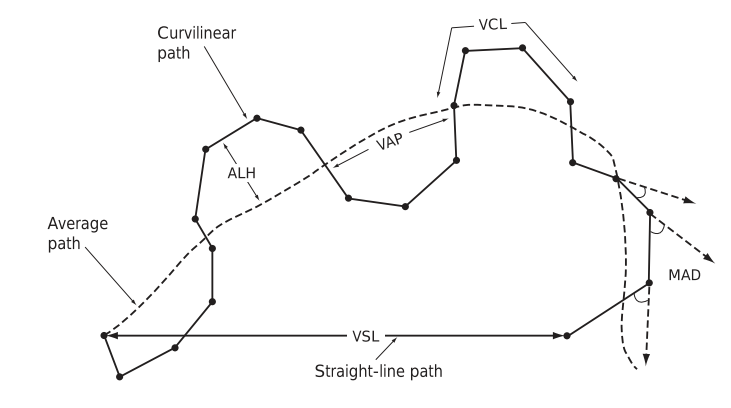
\includegraphics[width=5.5cm]{CASA.png}
  \end{subfigure}
  \caption{\textbf{Left} : Standard terminology for variables measured by CASA systems}
 \label{fig:CASA}
\end{figure}

Sperm Concentraion is measured with the help of a haemocytometer chamber and allowing it to settle.
The sperm sample needs to be well mixed and diluted and the slide needs to be covered by a cover slip and the results needs to be taken within 10-15 minutes to minimize the effects of evaporation.Morever 200 spermatozoa needs to be counted per replicate.
If the replicate counts are close they can be accepted otherwise we need to prepare new dilutions.After that the concentraions are calculated per ml.
haemocytometer has two separate counting chambers, 
each of which has a microscopic 3 mm × 3 mm pattern of 
gridlines etched on the glass surface. 
It is used with a special thick coverslip (thickness number 4, 0.44 mm), which lies over the grids and is supported by glass pillars 0.1 mm above the chamber fl oor. 
Each counting area is divided into nine 1 mm × 1 mm grids.

\begin{figure}[H]
  \centering
  \begin{subfigure}{5.5cm}
    \centering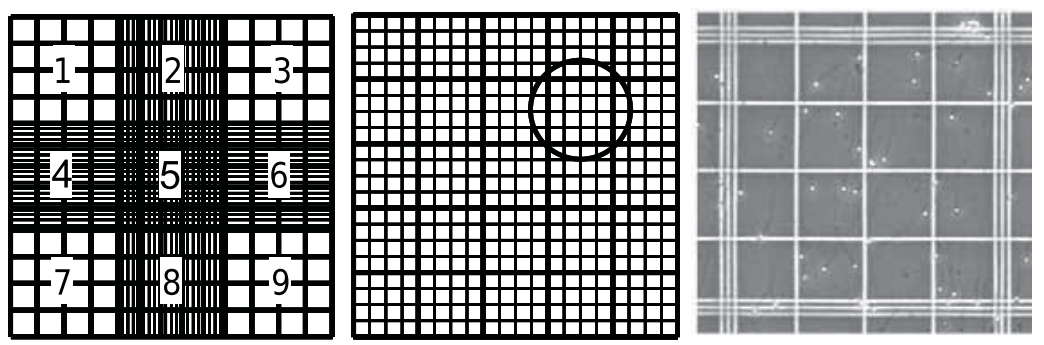
\includegraphics[width=6.5cm]{grid.png}
  \end{subfigure}
  \caption{\textbf{Left} : Sketches of the inscribed area showing: all nine grids in one chamber of the haemocytometer (left panel); the central grid (number 5) of 25 large squares (middle panel); and a micrograph of part of a fi lled chamber (right panel), showing one of the 25 squares of the central grid (the circled square in the middle panel) bounded by triple lines and containing 16 smaller squares.}
 \label{fig:grid}
\end{figure}


\section{Methods}

\textbf{Datasets}

In this project we used 4 videos for traning , 2 of the videos were taken directly from a sperm sample under a microscope covered under a cover slip.
While the other 2 sperm videos are taken from a sperm sample under a microscope in a glassslide along with the hemocytometer.All the samples have been taken from one individual.
Morever the validation data contains 1 data from the glass slide sample and one more data from the glass slide along with the hemocytometer. 
The validation data is used to tune the deep learning model while its training.

\begin{table}[H]
  \centering
  \begin{tabular}{|c|c|c|l}
  \cline{1-3}
  \begin{tabular}[c]{@{}c@{}}Data\\ type\end{tabular} &
    \begin{tabular}[c]{@{}c@{}}Sperm sample \\ on \\ glass slid\end{tabular} &
    \begin{tabular}[c]{@{}c@{}}Sperm sample on \\ glass slide \\ along with the \\ hemocytometer grid\end{tabular} &
     \\ \cline{1-3}
  TRAIN      & 2 & 2 &  \\ \cline{1-3}
  VALIDATION & 1 & 1 &  \\ \cline{1-3}
  TEST       & 1 & 6 &  \\ \cline{1-3}
  \end{tabular}
  \end{table}


\begin{figure}[H]
  \centering
  \begin{subfigure}{3.5cm}
    \centering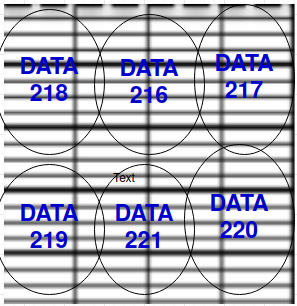
\includegraphics[width=3.5cm]{DL_grid.png}
  \end{subfigure}
  \caption{The videos taken from grid 4 to predict the sperm concentraion using deep learning methods}
 \label{fig:gradcam}
\end{figure}


\begin{figure}[H]
  \centering
  \begin{subfigure}{3.6cm}
    \centering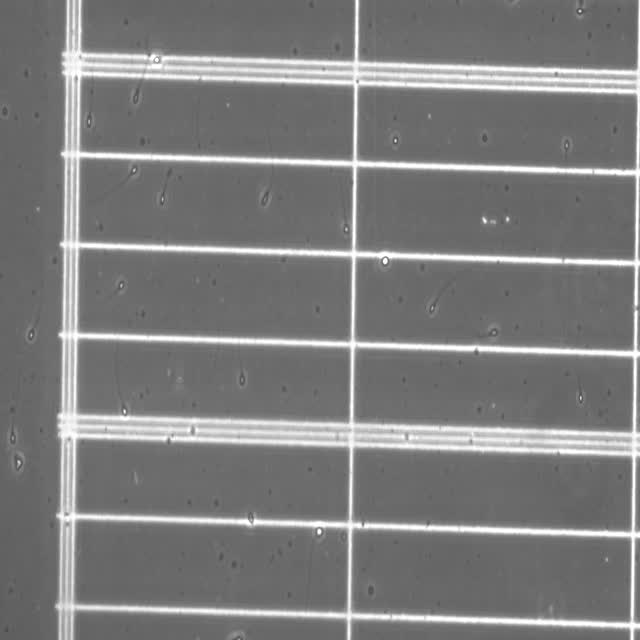
\includegraphics[width=3.6cm]{Data218_frame0.jpg}
  \end{subfigure}
  \begin{subfigure}{3.6cm}
    \centering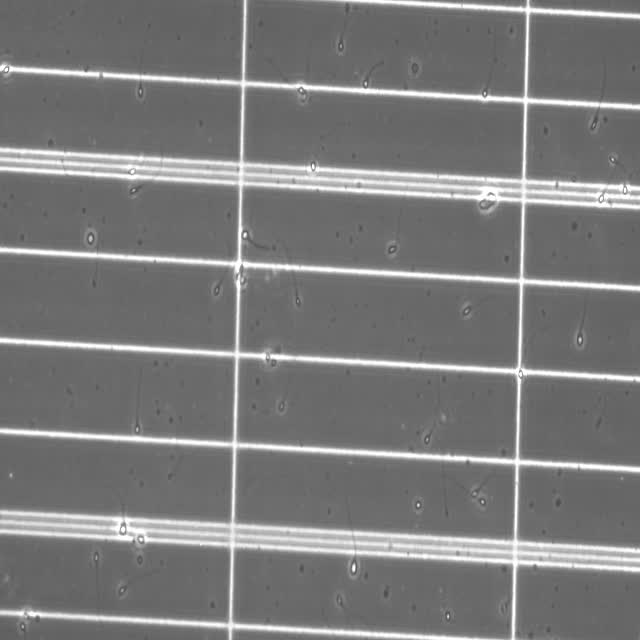
\includegraphics[width=3.6cm]{Data216_frame0.jpg}
  \end{subfigure}
  \begin{subfigure}{3.6cm}
    \centering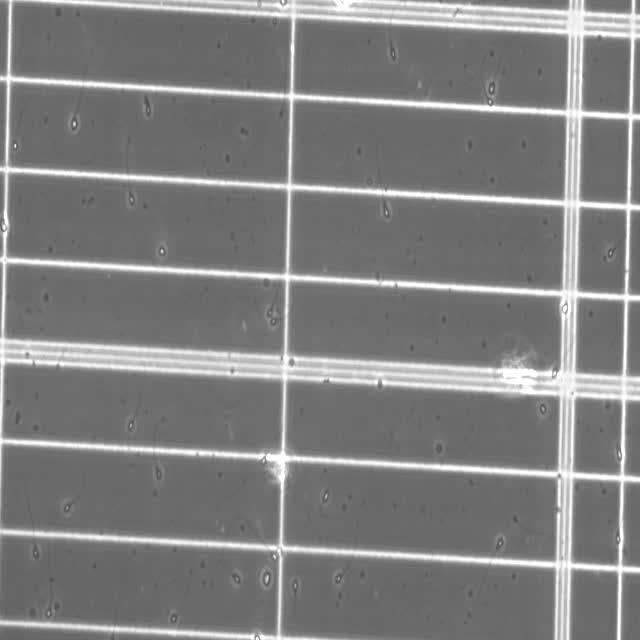
\includegraphics[width=3.6cm]{Data217_frame0.jpg}
  \end{subfigure}
  \\
  
  \begin{subfigure}{3.6cm}
    \centering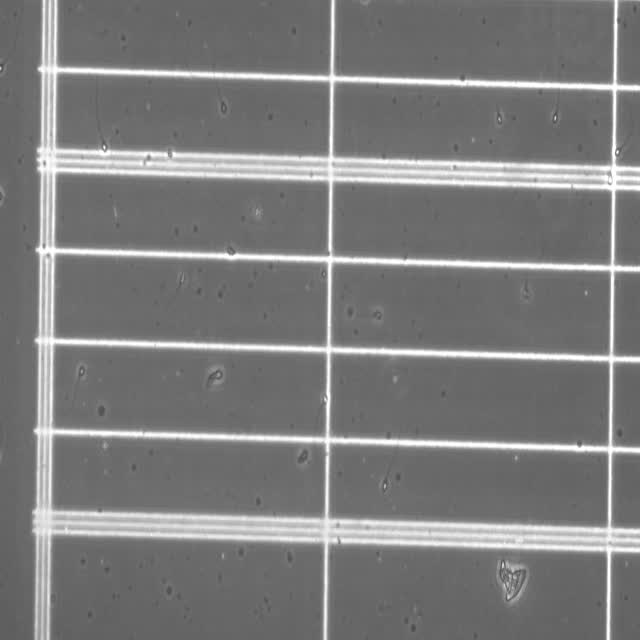
\includegraphics[width=3.6cm]{Data219_frame0.jpg}
  \end{subfigure}
  \begin{subfigure}{3.6cm}
    \centering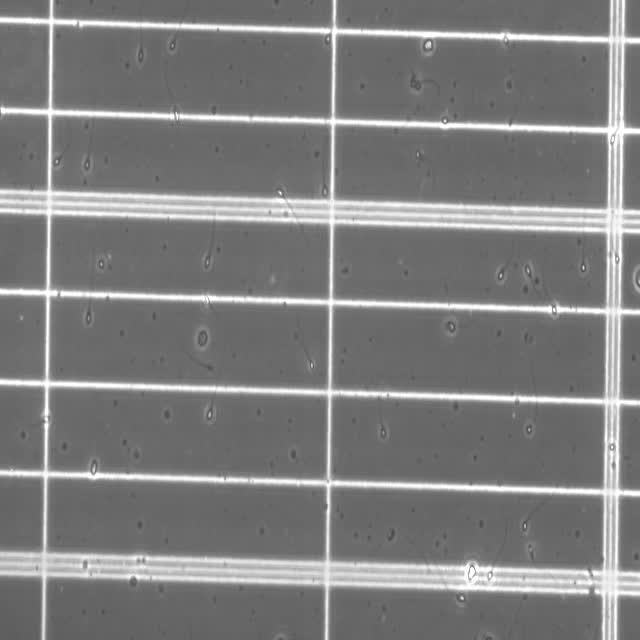
\includegraphics[width=3.6cm]{Data221_frame0.jpg}
  \end{subfigure}
  \begin{subfigure}{3.6cm}
    \centering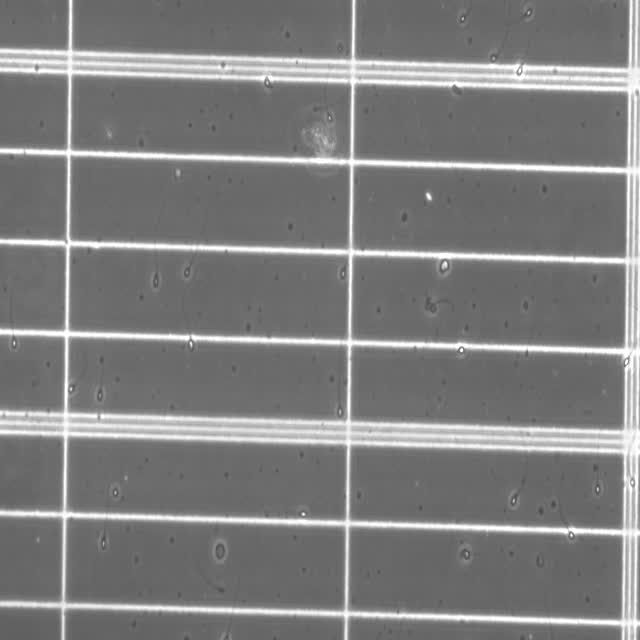
\includegraphics[width=3.6cm]{Data220_frame0.jpg}
  \end{subfigure}
  \caption{ 
  \textbf{Top}:First frame of the video of Data 218, 216 and 217.
  \textbf{Bottom} : First frame of the video of Data 219, 221 and 220.}
  \label{fig:cm_all}
\end{figure}

we annotated 4 sperm videos each of 3-5 seconds and it was taken at 30frames per second and we took 100 frames from each and we annoted the sperm heads in all of them.There were about 20-30 sperm heads on an average in each video.So a total of 
2000-3000 sperm were annotated and the sperm sample on glass slide along with the hemocytometer was used to predict the sperm concentraion while the sperm sample on the glass slides was used to predic the sperm motion.
The test data for the sperm concentraion contains 6 videos and each form an approximate part of the hemocytometer while the test data for the sperm motion contains data from the sperm sample taken from a glass slide.
The inital sperm concentration was very dense so we decided to go for a 1:5 dilution using PBS(phosphate-buffered saline ) and according to the WHO manual , grids 4,5,6 was used for counting the sperms and a minimum of 200 was counted in it with 15 rows in total.While it was difficult to take a video of grids 4,5 and 6 hence for the 
deep learning algorithm we decided to take only grid 4 as each videos were 1GB in size and data transfer was time consuming so we took 6 videos that provide an approximate overview of grid 4 which contains 5 rows.

The videos initally had the resoluton of $1920x1280$ , they were resized using a python script and made into the resolution of $640x640$ by cubic 
interpolation to minimize the model computaion memory and to maintain consistency between all the data.

\textbf{Models} 

For predicting the sperm concentration we decided to use the YOLOv5\citep{glenn_jocher_2021_5563715} algorithm , 
YOLO is an abbreviation for the term ‘You Only Look Once’. 
This is an algorithm that detects and recognizes various objects in a picture (in real-time). 
Object detection in YOLO is done as a regression problem and provides the class probabilities of the detected images.
YOLO algorithm employs convolutional neural networks (CNN) to detect objects in real-time. 
As the name suggests, the algorithm requires only a single forward propagation through a 
neural network to detect objects.This means that prediction in the entire image is done in a single algorithm run. 
The CNN is used to predict various class probabilities and bounding boxes simultaneously.
The YOLO algorithm consists of various variants. Some of the common ones include tiny YOLO, YOLOv3, YOLOv4 and YOLOv5. For the purpose of this study, we have chosen to go with YOLOv5 for the object detection.
\begin{figure}[H]
  \centering
  \begin{subfigure}{10.5cm}
    \centering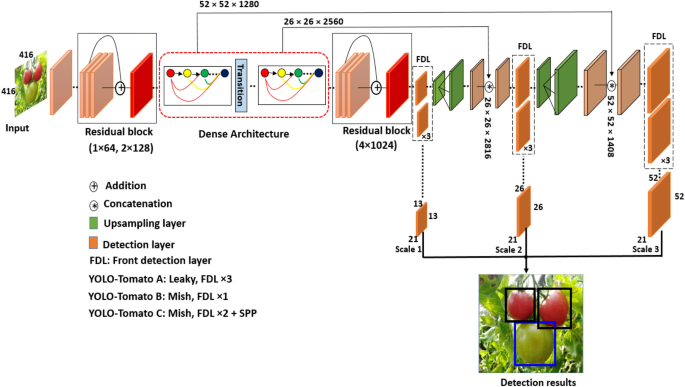
\includegraphics[width=10.5cm]{yolo.png}
  \end{subfigure}
  \caption{An example of the model used to create bounding boxes to detect fruits.In this case the bounding boxes would be created for the sperm heads.}
 \label{fig:yolo}
\end{figure}


\section{Results}

\textbf{Sperm Concentraion}

Using the yolo algorithm we predicted the sperm heads in each frame of the test set data containing the hemocytometer and took an average of the number of sperms in the video by counting the sperm heads in each frame and dividing the 
total number of frames which in this case is 100.


For the first case we manually calcuated the number of sperms in each of grids 4,5,6 using the method given below.
For 1:5 diluton \\ \\
Replicate 1 of total sperm count  = 228 \\
Replicate 2 of total sperm count  =  200 \\
Total number of rows($n$) $= 30(15 + 15)$ \\ 

Concentraion C is calcualted by the Formula : \\
$(N/(n)*(1/(v)))*(d)$ \\
where \\
N = Total number of sperm including the 2 replicas \\
n = total rows used for measurement \\
v = Volume of each row \\
d = dilution factor used \\

\begin{figure}[H]
  \centering
  \begin{subfigure}{4.6cm}
    \centering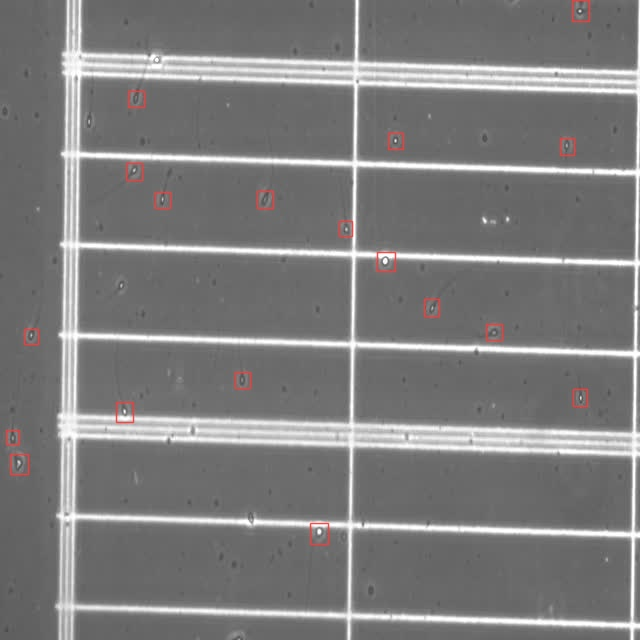
\includegraphics[width=4.6cm]{Data218_frame0_pred.jpg}
  \end{subfigure}
  \begin{subfigure}{4.6cm}
    \centering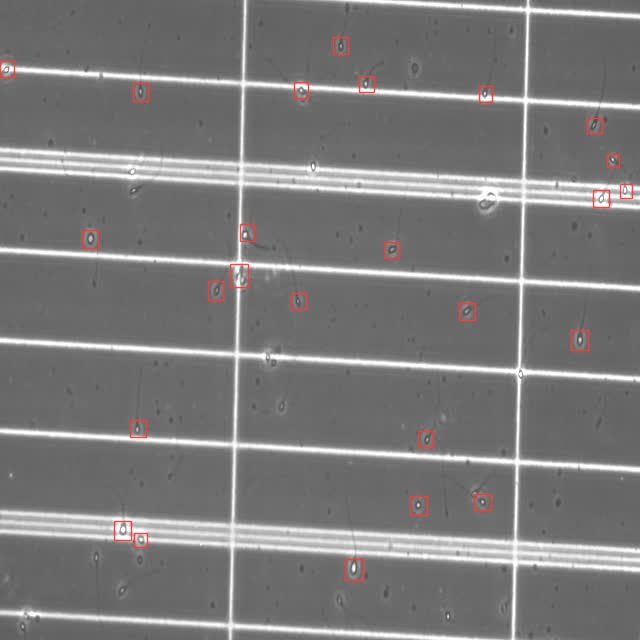
\includegraphics[width=4.6cm]{Data216_frame0_pred.jpg}
  \end{subfigure}
  \begin{subfigure}{4.6cm}
    \centering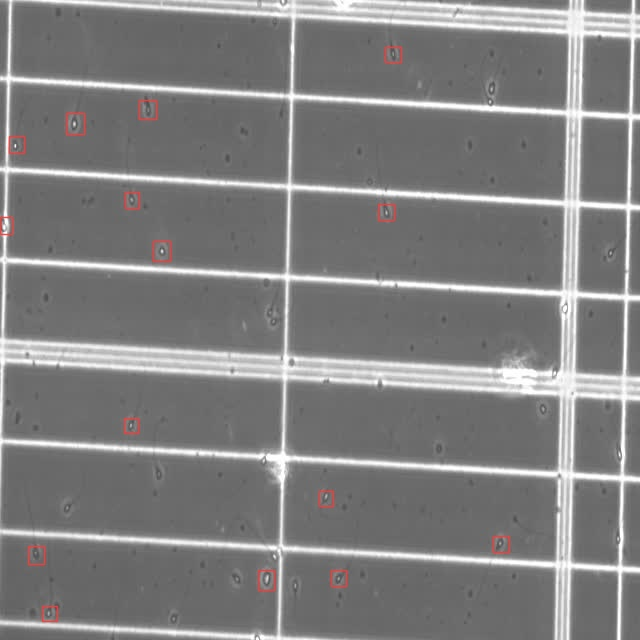
\includegraphics[width=4.6cm]{Data217_frame0_pred.jpg}
  \end{subfigure}
  \\
  
  \begin{subfigure}{4.6cm}
    \centering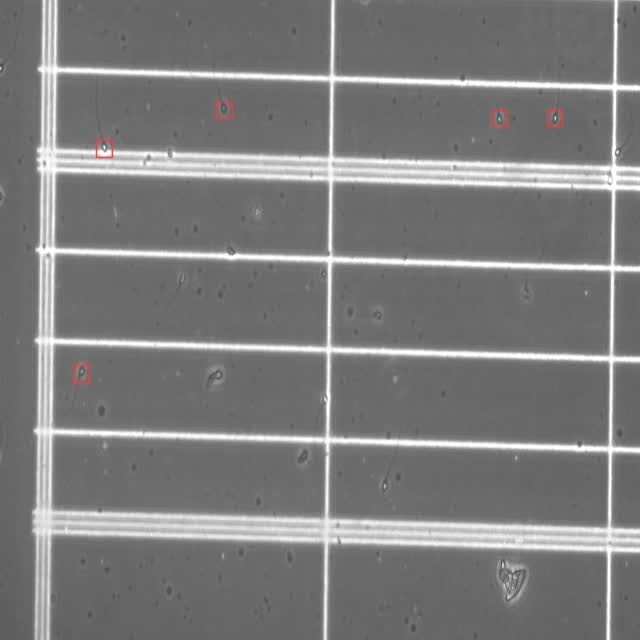
\includegraphics[width=4.6cm]{Data219_frame0_pred.jpg}
  \end{subfigure}
  \begin{subfigure}{4.6cm}
    \centering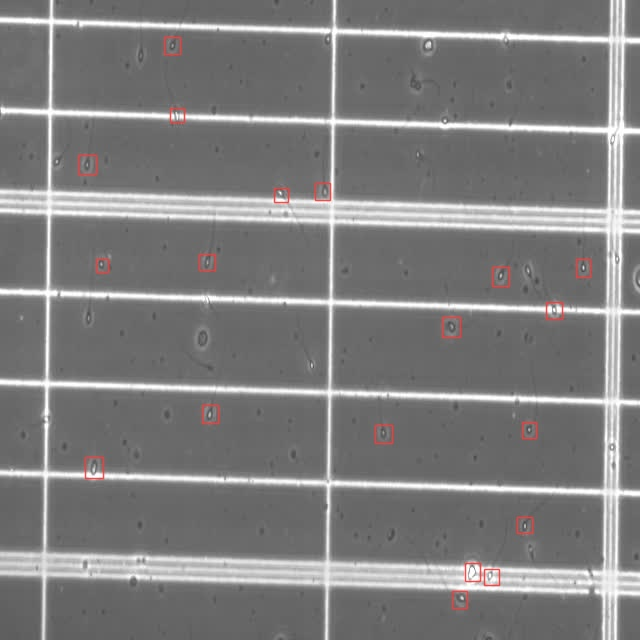
\includegraphics[width=4.6cm]{Data221_frame0_pred.jpg}
  \end{subfigure}
  \begin{subfigure}{4.6cm}
    \centering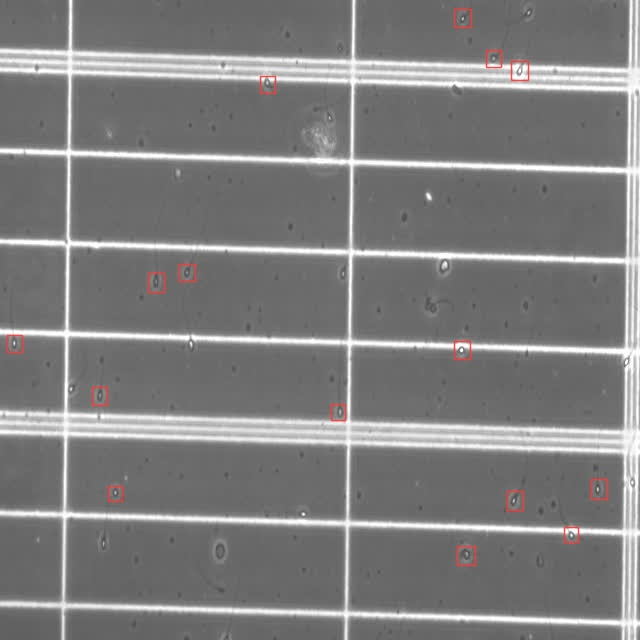
\includegraphics[width=4.6cm]{Data220_frame0_pred.jpg}
  \end{subfigure}
  \caption{ 
  \textbf{Top}:First frame of the predicted sperm heads in the video of Data 218, 216 and 217.
  \textbf{Bottom} : First frame of the predicted sperm heads in the video of video of Data 219, 221 and 220.}
  \label{fig:pred_video}
\end{figure}


Hence the calculation is : \\

$N = 228 + 200 = 428$ \\
$d = 5$ \\
$v = 20$ \\

$C = (428/30)*(1/20)*(5) $ \\
$C = 3.56/nl$ \\
Hence the concentration by manual Calculation is 3.56x$10^6$ sperms per milli litre
\\
To cross check if the values are correct or not , we take the difference between them \\
$228 - 220 = 28$ \\
\begin{figure}[H]
  \centering
  \begin{subfigure}{5.5cm}
    \centering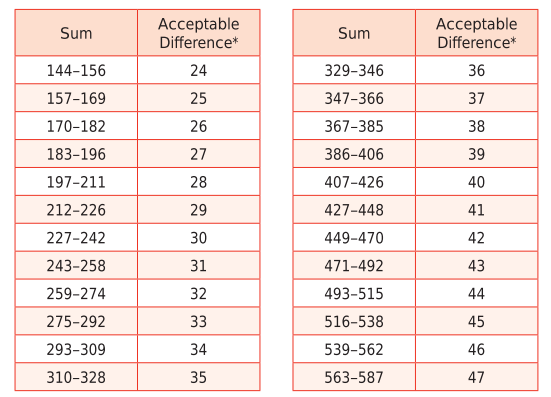
\includegraphics[width=5.5cm]{table.png}
  \end{subfigure}
  \caption{: Acceptable differences between two replicate counts for a given sum}
 \label{fig:gradcam}
\end{figure}
and we look up at the table and since the calculated different is less that the acceptalble difference , Hence
out values are correct. \\
We decided to use the same method to calculate the sperm concentration using the deep learning method .For this we decided to take a video of each of the 



Hence from this we got the following values: \\
Sperms in Data218 : 18 \\
Sperms in Data219 : 5 \\
Sperms in Data216 : 25 \\
Sperms in Data221: 19 \\
Sperms in Data217: 15 \\
Sperms in Data220: 15 \\
Total Sperms = 97 \\

For 1:5 diluton \\ \\
Total number of rows($n)= 5$ \\ 

Concentraion C is calcualted by the Formula : \\
$(N/(n)*(1/(v)))*(d)$ \\
where \\
N = Total number of sperm including the 2 replicas \\
n = total rows used for measurement \\
v = Volume of each row \\
d = dilution factor used \\

Hence the calculation is : \\

$N = 97$ \\
$d = 5$ \\
$v = 20$ \\

$C = (97/5)*(1/20)*(5) $ \\
$C = 4.85/nl$ \\
Hence the concentration by the Deep Learning method is 4.85x$10^6$ sperms per milli litre , since the total number of sperms in close to 100 hence the results would have a 
sampling error of 10\% according to the WHO manual.
\\

\textbf{Sperm Motion} 

For predicting the VCL and VSL for the top three most viable sperm , three videos of the sperm sample from the same individual were taken on a 
glass slide and two of the videos were annoted and trained and test on the third one.The current algorithm tracks the changes of the sperms present in the first frame to the last frame.


The algorithm goes through each frame and records the cordinates of each sperm in the frame as it traverses through the video 
If the distance between a sperm in frame $i$ to the frame $i+1$ is more than 0.05 then its a new sperm or the sperm went out of frame or it wasnt detected by the algorithm.
\begin{algorithm}[H]
  \caption{Sperm motin capture}\label{your_label}
  \begin{algorithmic}
    \STATE  initialize $SpermDictonary$ $\gets$  Contains the Cordinates of all the sperms of frame0 along with 
    their distances initialised to 0 in $total distance$.\\
      \FOR{ i = $1$ to $frameN$}
        \FOR{All $sperm_cordinates$ in  $frame[i]$}
          \STATE initialize $max$  $\gets$ $100$
          \FOR{ $key$ in  $SpermDictonary$}
            \STATE $distance$ = function to calculate distance between last cordinates of sperm in the $key$ and $sperm_cordinates$ 
            \IF { $distance$ $\leq$ $max$ }
              \STATE $max$ $\gets$ $distance$
              \STATE $index$ $\gets$ $key$
              \STATE $predictedx$  $\gets$ $x$
              \STATE $predictedy$  $\gets$ $y$
            \ENDIF
          \ENDFOR
          \IF { $max$ $\leq$ $0.05$ } 
          \STATE  Append the sperm in the  $SpermDictonary$ with the new cordinate and add $max$ to the $total distance$. 
          \ENDIF
          \ENDFOR
        \ENDFOR
  \end{algorithmic}
\end{algorithm}


\begin{figure}[H]
  \centering
  \begin{subfigure}{4.6cm}
    \centering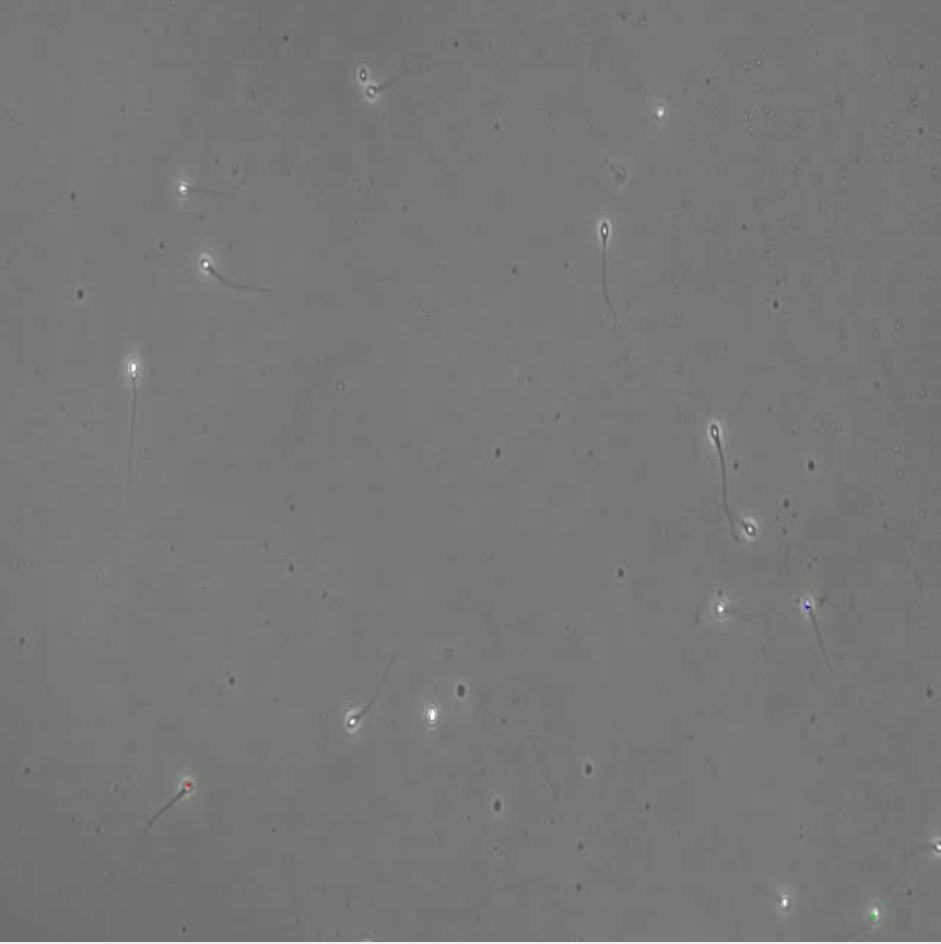
\includegraphics[width=4.6cm]{frame_0.png}
  \end{subfigure}
  \begin{subfigure}{4.6cm}
    \centering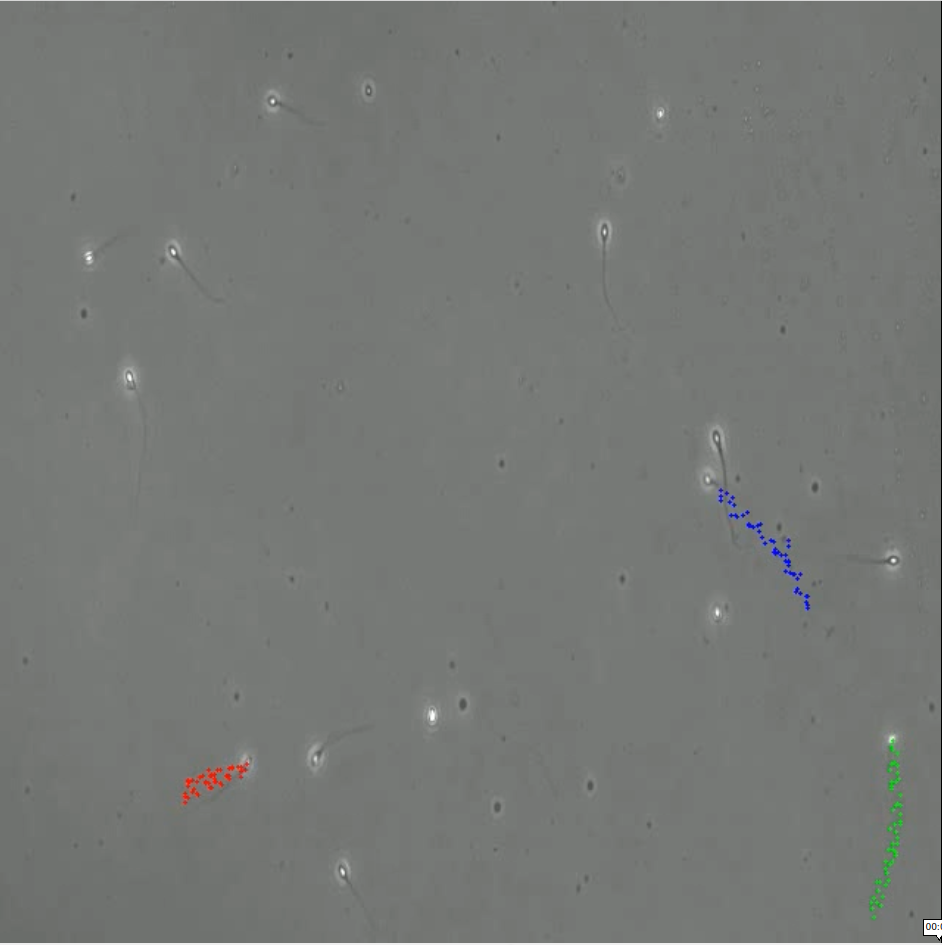
\includegraphics[width=4.6cm]{frame_50.png}
  \end{subfigure}
  \begin{subfigure}{4.6cm}
    \centering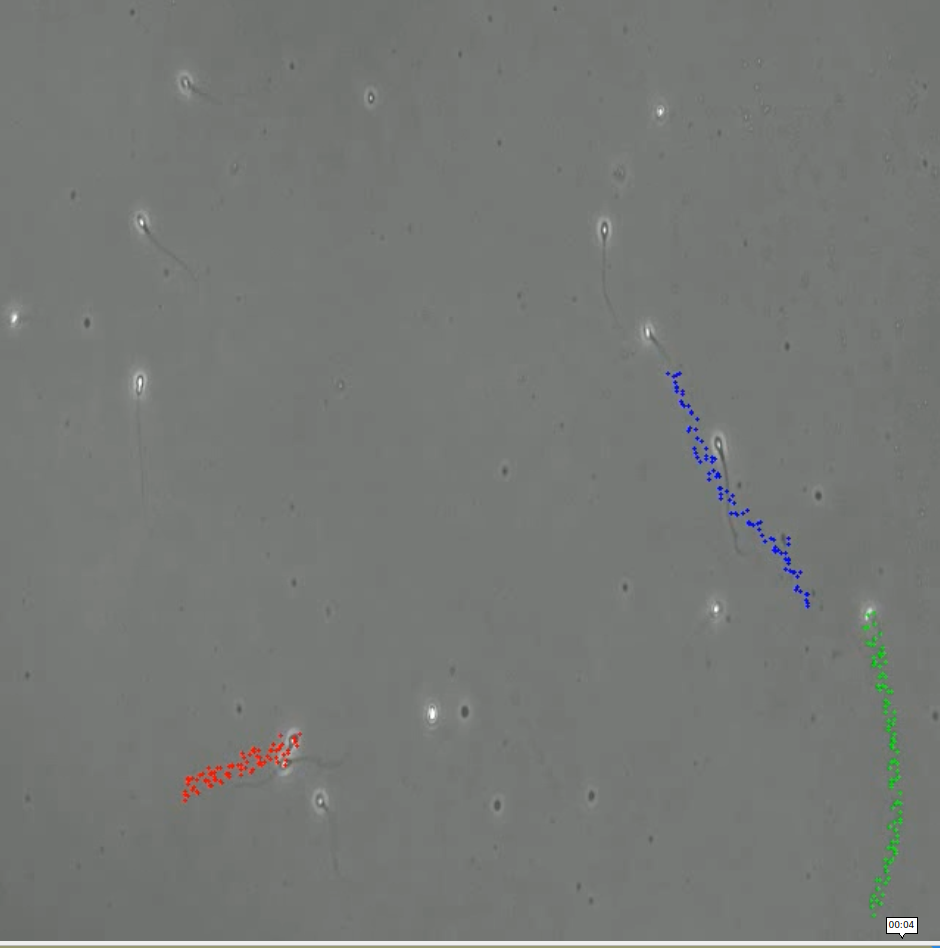
\includegraphics[width=4.6cm]{frame_100.png}
  \end{subfigure}
  \caption{ 
  \textbf{Left}:Tracked motion of the top 3 sperms in frame 0,
  \textbf{Center} : Tracked motion of the top 3 sperms in frame 50,
  \textbf{Right} : Tracked motion of the top 3 sperms in frame 100}
  \label{fig:pred_video_motion}
\end{figure}
Each pixel in the frame was considered to be 0.5 microns and let the Top 3 viable sperms be named as sperm red, blue and green. \\
\begin{table}[H]
  \centering
  \begin{tabular}{|c|c|c|l}
  \cline{1-3}
  Sperm type & \begin{tabular}[c]{@{}c@{}}VCL(in micrometer \\ per second)\end{tabular} & \begin{tabular}[c]{@{}c@{}}VSL(in micrometer \\ per second)\end{tabular} &  \\ \cline{1-3}
  Red   & 94.63 & 9.06  &  \\ \cline{1-3}
  Green & 68.29 & 33.3  &  \\ \cline{1-3}
  Blue  & 81.94 & 36.14 &  \\ \cline{1-3}
  \end{tabular}
  \end{table}

  \section{Conclusion}
  Through this study we tend to show that deep learning tool can be used to predict parameters of sperm viablity.
  These results should be still considered as preliminary until wide scale generalizability of these models are established. 
  This study provides a proof of concept that needs careful consideration before clinical implementation. 
  It should be noted that application of these models should be limited to helping the clinical team in decision making, 
  and not to replace their role entirely. 

  \section{Future Work}
  For our current study we have worked with only one subject hence multi subject studies can improve the generalizability of the models , morever the sperm motion algorithm may fail to detect sperms
  that enter after the first frame and this has to be improved , morever we cannot always relay on the model to predict the sperm heads at all times hence a fail safe needs to be implemented such that the algorithm can track the sperm head even if the model didnt detect it based on 
  the previous frames and successive frames. \\
  Morever our model currently uses only the sperm head , this could be expanded to include the dynamics of the tail which could help in improving the predictability of sperm motion and dynamics.
  We also provide the data for the annotated frames so that future researchers can continue on the project.
  \bibliography{references}


\end{document} 
